\documentclass{article}

\usepackage{graphicx}
\usepackage{amsmath}
\usepackage{float}

\title{PA3: Priority Queues and Heaps}
\author{Kevin Lei}
\date{March 22, 2024}

\begin{document}

\maketitle

\section{Introduction}
This assignment aims to implement a priority queue using three different methods: an array representation of a binary heap, a sorted array, and an unsorted array. 
In this report, we will discuss the theoretical time complexities for the enqueue operation and heap sort for each of these methods. 
Additionally, we will describe an experiment designed to gather evidence supporting the theoretical time complexities. 
Finally, we will compare and contrast the results obtained from each implementation to gain a better understanding of how the choice of data structure affects the performance of a priority queue in terms of time complexity and practical implementation.

\section{Theoretical Analysis}
Here we will discuss the theoretical time complexities for the enqueue operation and heap sort for the binary heap, sorted array, and unsorted array implementations of a priority queue. 
It's important to note that all implementations use an array and need to be resized when the array is full. 
The resizing is done by copying over all existing elements to an array double the size of the old array.

\subsection{Binary Heap}
\subsubsection{Enqueue Operation}
The enqueue operation for the binary heap has a best case time complexity of $O(1)$ when the element to be inserted is the maximum element in the heap (since the heap implemented is a min-heap). 
On average, and in the worst case, the time complexity is $O(\log n)$, since the element may need to be bubbled up to the correct position in the heap up to the height of the heap, which is $\log n$. 
The resizing operation, which occurs when the array is full, takes $O(n)$ time. 
However, since the array size doubles each time, the amortized cost of resizing is $O(1)$ per insertion.

\subsubsection{Heap Sort}
In all cases, the time complexity of heap sort with the binary heap implementation is $O(n \log n)$. 
Even when elements are inserted into the heap in sorted order, the time complexity remains $O(n \log n)$, as heapify will still take $O(\log n)$ time for each element, resulting in a total time complexity of $O(n \log n)$. 
If the elements are inserted in random or reverse sorted order, the time complexity is still $O(n \log n)$. 
Inserting $n$ elements will take $O(n \log n)$ time, and removing the elements will take $O(n \log n)$ time, resulting in a total time complexity of $O(n \log n)$. 
The resizing operation during insertion has an amortized cost of $O(1)$ per insertion, so it doesn't affect the overall time complexity.

\subsection{Sorted Array}
\subsubsection{Enqueue Operation}
The best case time complexity of the enqueue operation for a sorted array is $O(1)$ when the element to be inserted is the maximum element in the array. 
On average, and in the worst case, the time complexity is $O(n)$, since the element may need to be inserted at the end of the array and then shifted to the correct position in the array up to the length of the array, which is $n$. 
The resizing operation takes $O(n)$ time, but since it occurs only when the array is full, the amortized cost of resizing is $O(1)$.

\subsubsection{Heap Sort}
In all cases, the time complexity of heap sort with the sorted array implementation is $O(n^2)$. 
This is because no matter the order in which elements are inserted, the time complexity of removing the elements is $O(n^2)$, as $n$ removals will take $O(n)$ time each. 
Like before, the resizing operation during insertion has an amortized cost of $O(1)$.

\subsection{Unsorted Array}
\subsubsection{Enqueue Operation}
The time complexity of the enqueue operation for an unsorted array is $O(1)$ in all cases, since the element is simply appended to the end of the array. 
The resizing operation here once again has an amortized cost of $O(1)$ per insertion.

\subsubsection{Heap Sort}
The time complexity of heap sort with the unsorted array implementation will always be $O(n^2)$. 
This is because inserting $n$ elements will take $O(n)$ time, and removing the elements will take $O(n^2)$ time, since $n$ elements need to be removed and the minimum element needs to be found each time, and each removal will take $O(n)$ time. 
The resizing operation during insertion has an amortized cost of $O(1)$ per insertion, so it doesn't affect the overall time complexity.

\section{Experimental Setup}
To gather experimental evidence supporting the theoretical time complexities, we designed an experiment that measures the running time of the enqueue operation and heap sort for each priority queue implementation. 
The test inputs were generated using a random number generator, producing integers in the range $[0, 100000)$. 
We tested the following input sizes: 1000, 5000, 10000, 50000, and 100000. 

\section{Experimental Results}
The experimental results are presented in the form of graphs comparing the running times of the enqueue operation and heap sort for each priority queue implementation.

\begin{figure}[H]
    \centering
    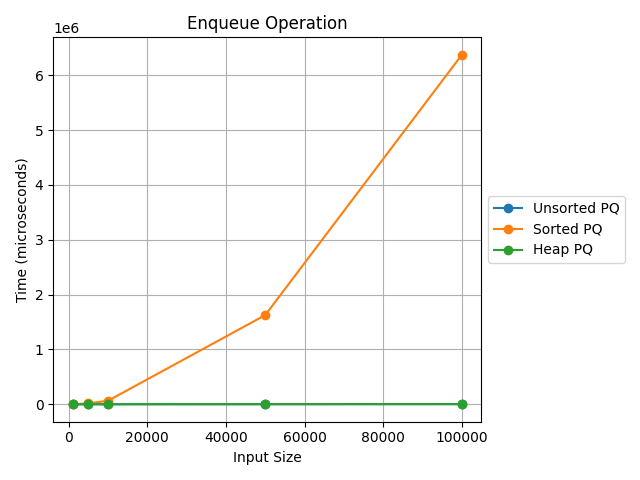
\includegraphics[width=0.8\textwidth]{../plots/enqueue_linear.png}
    \caption{Running times of the enqueue operation on a linear scale.}
\end{figure}

Looking at Figure 1, it is evident that the unsorted array implementation performs the best, with a nearly constant running time across all input sizes. 
The binary heap implementation shows a logarithmic growth in running time, while the sorted array implementation shows a linear increase in running time as the input size grows.

\begin{figure}[H]
    \centering
    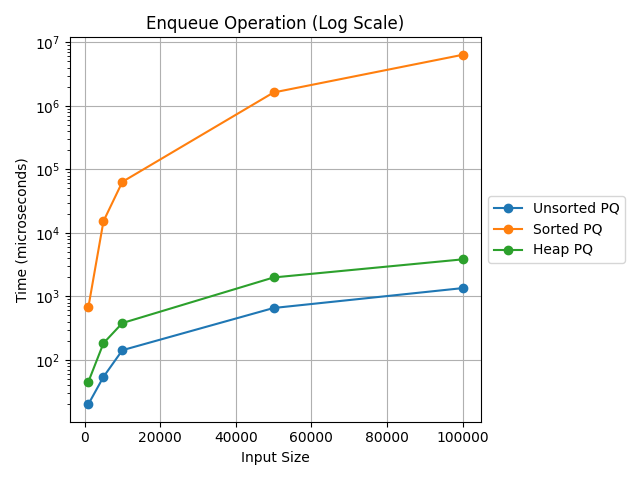
\includegraphics[width=0.8\textwidth]{../plots/enqueue_log.png}
    \caption{Running times of the enqueue operation on a logarithmic scale.}
\end{figure}

Figure 2 presents the same data as Figure 1 but on a logarithmic scale. 
This plot highlights the differences in growth rates more clearly. 
The unsorted array and binary heap implementations have a relatively slow growth rate, while the sorted array implementation grows more rapidly.

\begin{figure}[H]
    \centering
    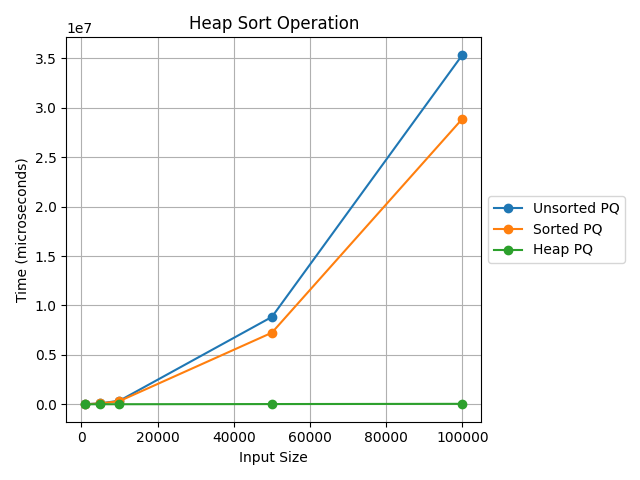
\includegraphics[width=0.8\textwidth]{../plots/heapsort_linear.png}
    \caption{Running times of the heap sort operation on a linear scale.}
\end{figure}

Looking at Figure 3, the binary heap implementation outperforms the other two, with a running time that grows slowly with increasing input size. 
The unsorted array and sorted array implementations both exhibit quadratic growth in running time, with the unsorted array being slightly faster.

\begin{figure}[H]
    \centering
    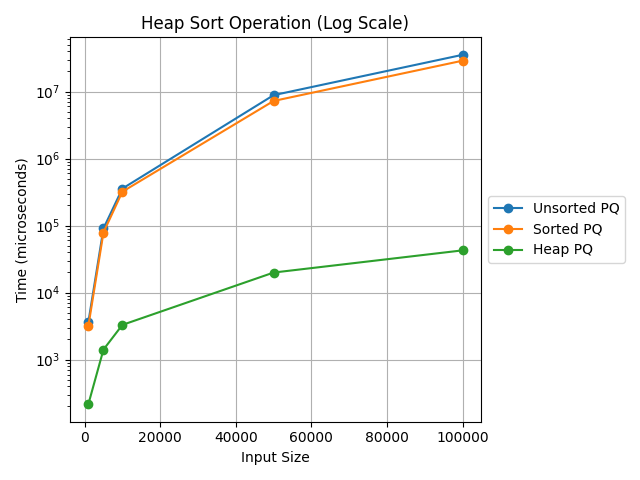
\includegraphics[width=0.8\textwidth]{../plots/heapsort_log.png}
    \caption{Running times of the heap sort operation on a logarithmic scale.}
\end{figure}

Figure 4 shows the heap sort running times on a logarithmic scale, emphasizing the different growth rates. 
The binary heap implementation has a logarithmic growth rate, while the unsorted array and sorted array implementations have a nearly quadratic growth rate.

The experimental results align well with the theoretical analysis. 
The unsorted array provides the best performance for the enqueue operation, with a constant time complexity of $O(1)$. 
The binary heap has a logarithmic time complexity of $O(\log n)$ for enqueue, which is reflected in its slower growth rate compared to the unsorted array. 
The sorted array has a linear time complexity of $O(n)$ for enqueue, which is evident in its linear growth in running time.

For the heap sort operation, the binary heap implementation demonstrates the best performance, with a time complexity of $O(n \log n)$. 
This is supported by the experimental results, where the binary heap exhibits a logarithmic growth rate. 
The unsorted array and sorted array implementations both have a quadratic time complexity of $O(n^2)$ for heap sort, which is confirmed by their nearly quadratic growth rates in the experimental results.

In conclusion, the experimental results provide strong evidence supporting the theoretical time complexities of the enqueue operation and heap sort for each priority queue implementation. 
The binary heap offers the best overall performance, particularly for the heap sort operation, while the unsorted array is the most efficient for the enqueue operation. 
The sorted array implementation performs poorly in both cases due to its linear time complexity for enqueue and quadratic time complexity for heap sort.

\end{document}